\documentclass[conference]{IEEEtran}
\IEEEoverridecommandlockouts

\usepackage{amsmath,amssymb}
\usepackage{graphicx}
\usepackage{cite}
\usepackage{booktabs}
\usepackage{array}
\usepackage[table]{xcolor}
\usepackage{url}
\usepackage{hyperref}
\usepackage{pifont}

\newcolumntype{L}[1]{>{\raggedright\arraybackslash}p{#1}}
\newcolumntype{C}[1]{>{\centering\arraybackslash}p{#1}}

% ---- palette (matches the paper's figures; validated print/grayscale-safe) ----
\definecolor{headerfill}{HTML}{DBE9FA}
\definecolor{headertext}{HTML}{104281}
\definecolor{rowstripe}{HTML}{F6F8FB}
\definecolor{ruleblue}{HTML}{2A78D6}
\definecolor{cgood}{HTML}{0CA30C}
\definecolor{ccrit}{HTML}{D03B3B}
\renewcommand{\arraystretch}{1.18}
\newcommand{\okmark}{\textcolor{cgood}{\checkmark}}
\newcommand{\badmark}{\textcolor{ccrit}{\textbf{\ding{55}}}}

\begin{document}

\title{NyayaOS: Confidence-Aware Multi-Source Synchronization for Justice Digital Twins}

\author{
\IEEEauthorblockN{Khushi Shetty}
\IEEEauthorblockA{Department of Computer Science \& Engineering\\
Dayananda Sagar College of Engineering\\
Bangalore, India\\
khushishetty053@gmail.com}
\and
\IEEEauthorblockN{Isha Rajmohan}
\IEEEauthorblockA{Department of Computer Science \& Engineering\\
Dayananda Sagar College of Engineering\\
Bangalore, India\\
isha.rajmohan1@gmail.com}
\and
\IEEEauthorblockN{Dhravya Shetty}
\IEEEauthorblockA{Department of Computer Science \& Engineering\\
Dayananda Sagar College of Engineering\\
Bangalore, India\\
dhravyashetty285@gmail.com}
}

\maketitle

\begin{abstract}
A legal case is not produced by a single record-keeper. Police, courts,
lawyers, and forensic agencies each generate case information independently
and at different times, and no one source is authoritative for every fact
about a case. Existing legal information systems support document storage,
retrieval, and question answering over this material, but they treat each
document as an independent artifact rather than as one more observation of a
case whose state must be kept internally consistent as new, sometimes
conflicting, sometimes delayed information arrives. This paper presents
NyayaOS, a case-centric Justice Digital Twin architecture, and its central
mechanism, Confidence-Aware Multi-Source Synchronization (CAMS). CAMS
evaluates every incoming observation against the existing case record using
four factors --- source authority, temporal consistency, cross-source
corroboration, and extraction reliability --- combines them into a single
confidence score, and applies a threshold-and-margin rule to decide whether
the synchronized case state should be updated, retained unchanged, or left
unresolved pending further evidence. Observations are never discarded or
overwritten: every incoming record and every synchronization decision is
stored, giving each synchronized fact a traceable provenance chain back to
the evidence that produced it. We verified the implementation against its
source code rather than against the project's own description of itself,
and evaluated it through (i) an end-to-end pipeline execution over a
hand-built case scenario, (ii) a controlled comparison of CAMS, four
single-factor ablations of CAMS, and three simpler synchronization baselines
across five scenario types (conflicting, delayed, noisy, corroborating, and
duplicate observations), and (iii) a threshold/margin sensitivity sweep.
Across these controlled scenarios, CAMS matched the intended reference
outcome in 4 of 5 cases; removing any one of the temporal, corroboration, or
extraction-reliability factors caused it to fail exactly the scenario
designed to exercise that factor, while a naive latest-observation-wins
baseline failed 3 of 5. These results describe execution behavior on a
small, hand-authored evaluation, not generalizable accuracy, real-world
robustness, or legal correctness, and they are reported at the scale that
was actually implemented and run, not the scale of a production deployment.
\end{abstract}

\begin{IEEEkeywords}
Justice Digital Twin, Legal Information Systems, Multi-Source Information
Fusion, Conflict Resolution, Confidence-Aware Synchronization, Temporal
Information Processing, Legal AI.
\end{IEEEkeywords}

\section{Introduction}
\label{sec:introduction}

Judicial processes generate case information continuously and from many
independent places at once. A single criminal case can accumulate a police
first-information report, one or more witness statements, forensic findings,
a sequence of court orders, and communications from lawyers on both sides,
each produced by a different institution on its own schedule. None of these
records is inherently more current than the others, and none is guaranteed
to agree with the rest: a forensic report may arrive weeks after the event
it describes, two witnesses may recall an incident's timing differently, and
a police record and a court order may temporarily disagree about a
defendant's custody status simply because they were filed at different
points in the same unfolding process. The result is that the true state of a
case --- who is in custody, what has been established about an incident,
what a court has most recently ordered --- exists only implicitly, scattered
across documents that were never designed to be read together.

Conventional legal information systems address part of this problem.
Document management, retrieval, and question-answering tools make it
possible to locate and read the individual records that make up a case.
They do not, by themselves, solve a different problem: deciding what a
case's current state \emph{is} when its records disagree, arrive out of
order, repeat each other, or vary in how reliably they were digitized.
Storing and retrieving documents is a necessary condition for a usable case
record; it is not sufficient for maintaining one continuously updated
representation of the case that reflects the best available synthesis of
everything received so far. That synthesis problem --- deciding, each time a
new observation arrives, whether it should change the case's recorded
state, and keeping an auditable account of why --- is what this paper calls
multi-source synchronization, and it is distinct from extraction or
retrieval even though it depends on both.

Digital Twin architectures offer a conceptual vocabulary for this problem: a
continuously updated digital representation of an evolving real-world
entity, kept synchronized as new information about that entity arrives.
Applying this idea to a legal case is natural --- the case \emph{is} an
evolving entity with parties, events, evidence, and proceedings --- but a
Justice Digital Twin cannot be built by simply storing the newest record for
each fact and discarding the rest. Two records reporting different values
for the same fact are not automatically a case where the newer one is
correct; a delayed report about an earlier event is not evidence that the
event happened later; and a fact repeated by three copies of the same
underlying source should not be treated as more corroborated than one
confirmed independently by three different institutions. General
multi-source information fusion research has developed principled ways to
combine heterogeneous, uncertain observations from multiple sources, and
legal AI research has produced strong tools for extracting structured
information from legal text. Neither literature, on its own, is organized
around the specific requirement this paper addresses: synchronizing a
continuously evolving, multi-source legal case record while explicitly
accounting for which source is authoritative for which kind of fact, whether
an event's reported timing is consistent with the case's known chronology,
whether a value is corroborated by independent sources rather than repeated
by one, and how much extraction uncertainty a given observation carries ---
together, and with every decision traceable back to the evidence that
produced it.

This paper presents NyayaOS, a case-centric Justice Digital Twin
architecture, and Confidence-Aware Multi-Source Synchronization (CAMS), the
mechanism at its core. CAMS treats every incoming piece of case information
as an observation rather than as a direct edit to the case record. Before an
observation is allowed to change the synchronized state, CAMS scores it ---
and any observations it competes with --- on source authority, temporal
consistency, cross-source corroboration, and extraction reliability,
combines these into a single confidence value, and applies a configurable
threshold and margin to decide whether the case state should be updated,
retained as-is, or marked unresolved. Observations are never deleted or
overwritten regardless of the outcome, so the synchronized state can always
be traced back to the specific observations and the specific synchronization
decision that produced it.

This paper evaluates whether that mechanism behaves as intended on a small,
controlled, hand-authored set of scenarios: a working end-to-end pipeline
execution, a comparison of CAMS against its own single-factor ablations and
against three simpler baseline synchronization rules across five scenario
types, and a sensitivity analysis of the mechanism's two decision
parameters. It does not evaluate CAMS against a real or independently
annotated legal dataset, does not measure legal or forensic accuracy in any
sense, and does not evaluate the document-extraction pipeline against real
scanned or heterogeneous case documents --- the working implementation, as
verified against its source code, processes text-bearing PDFs and does not
yet include an OCR path for scanned documents. Nothing in this paper should
be read as a claim that NyayaOS determines legal facts, assesses evidentiary
admissibility, or makes or informs a judicial decision; CAMS's confidence
score governs only whether the \emph{digital twin representation} is
updated, not any legal conclusion.

The contributions of this paper are:

\begin{enumerate}
\item CAMS, a confidence-aware synchronization mechanism that scores
competing observations of the same case fact on source authority, temporal
consistency, cross-source corroboration, and extraction reliability, and
applies a threshold-and-margin decision rule to update, retain, or leave a
case fact unresolved, implemented and verified against its own test suite
and a working execution pipeline.
\item An append-only, provenance-preserving data model that separates raw
observations from the synchronized Justice Digital Twin state, so that
every synchronized fact remains traceable to the observations and the
synchronization decision that produced it, and so that competing or
unresolved information is never silently lost.
\item A controlled comparative evaluation --- CAMS against four
single-factor ablations of itself and three simpler synchronization
baselines, across five scenario types, together with a threshold/margin
sensitivity analysis --- reported at the scale it was actually run, with
every number traceable to a saved, reproducible execution log.
\end{enumerate}

\section{Related Work and Research Gap}

Research on digital technologies in judicial environments has identified
Digital Twins as a plausible way to represent complex court and justice
processes, motivating the general idea of a continuously maintained digital
counterpart to a real-world case \cite{bhatt2024}. This literature
establishes the case for building such a representation but does not itself
specify a mechanism for keeping it synchronized when the observations
feeding it are heterogeneous, delayed, or mutually inconsistent --- the
problem this paper addresses.

A separate body of legal AI research has focused on extracting structure
from legal text and reasoning over it once extracted: legal case analysis,
information extraction, argument mining, and judgment prediction have all
been investigated directly. LegalAsst demonstrates a human-centered,
AI-assisted system for structured legal information processing and court
productivity \cite{han2024}. Yue et al. propose an explainable,
circumstance-aware framework for legal judgment prediction \cite{yue2024}.
Castano et al. develop context-aware techniques for enforcing structured
legal information extraction from text \cite{castano2024}. Habernal et al.
mine legal arguments directly from court decisions \cite{habernal2024}.
These systems make a strong case that individual legal documents can be
turned into structured, usable information, and CAMS depends on exactly
this kind of extraction as its input. None of them, however, addresses what
happens when structured observations \emph{about the same fact} arrive from
more than one such extraction process and disagree --- extraction quality
and synchronization are different problems, and solving the first does not
solve the second.

Multi-source information fusion research addresses the second problem
directly, but at a level of generality that does not carry the specific
structure of a legal case. Li et al. survey progress and open problems in
combining heterogeneous, uncertain information from multiple sources in
general terms \cite{li2024}; Jiao reviews methods for fusing uncertain
information more broadly \cite{jiao2024}. These works are the
methodological ancestors of CAMS's confidence-fusion approach --- the idea
of scoring and combining evidence from multiple sources under uncertainty
is not new, and this paper does not claim otherwise --- but neither is
formulated around case-specific structure such as fact-dependent source
authority, an explicit separation between when an event occurred and when
it was reported, or a provenance requirement tying every synchronized value
back to the evidence and decision that produced it.

A third relevant strand concerns explainability, fairness, and
accountability in legal AI, which motivates why a synchronization mechanism
for legal information should not behave as an opaque or self-certifying
oracle. Bex situates AI-and-law research within a transdisciplinary
ecosystem and argues for systems that remain legible to the people affected
by them \cite{bex2025}. Papagianneas and Junius examine fairness and
automation in the specific context of smart courts \cite{papagianneas2023}.
Pfeiffer et al. offer an interdisciplinary view of algorithmic fairness
relevant to systems deployed in consequential domains \cite{pfeiffer2023}.
None of these proposes a synchronization algorithm, but together they
motivate two design commitments that shape CAMS: that a confidence score
used to decide whether to update a digital case representation must not be
conflated with a legal or evidentiary judgment, and that every
synchronization decision should be traceable to the evidence that produced
it rather than presented as a black-box output.

Table \ref{tab:relatedwork} summarizes this positioning. Taken together,
this literature supports the individual pieces NyayaOS depends on --- the
idea of a Justice Digital Twin, methods for extracting structured legal
information, general approaches to multi-source fusion, and the case for
explainable and accountable legal AI --- but does not, individually or
collectively, provide a synchronization mechanism designed around the
specific requirements of an evolving, multi-source legal case record:
fact-dependent source authority, an explicit separation of event time from
ingestion time, corroboration measured across independent source groups
rather than independent documents, and a provenance trail linking every
synchronized value back to specific evidence. That gap --- not the
existence of Digital Twins, legal AI, or information fusion as fields,
which are well established --- is what CAMS is scoped to address.

\begin{table*}[t]
\centering
\caption{Related work and how it relates to CAMS's scope}
\label{tab:relatedwork}
\rowcolors{2}{rowstripe}{white}
\begin{tabular}{L{2.6cm}L{5.2cm}L{8.5cm}}
\toprule
\rowcolor{headerfill}
\textcolor{headertext}{\textbf{Author(s)}} & \textcolor{headertext}{\textbf{Methodology}} & \textcolor{headertext}{\textbf{Relation to this work}} \\
\midrule
Bhatt et al. \cite{bhatt2024} & Justice Digital Twin and Industry 4.0 review & Motivates the Digital Twin framing; does not specify a synchronization mechanism \\
Han et al. \cite{han2024} & AI-assisted legal case analysis (LegalAsst) & Structured legal information processing; single-source, not multi-source conflict handling \\
Yue et al. \cite{yue2024} & Explainable legal judgment prediction & Prediction-focused; not concerned with case-state synchronization \\
Li et al. \cite{li2024} & Multi-source information fusion (general) & Methodological basis for confidence fusion; not legal-case-specific \\
Jiao \cite{jiao2024} & Uncertain information fusion (general) & Same relation as \cite{li2024}; general-purpose, not case-structured \\
Castano et al. \cite{castano2024} & Context-aware legal information extraction & Supplies the kind of structured input CAMS consumes; extraction only \\
Habernal et al. \cite{habernal2024} & Legal argument mining & Reasoning over extracted arguments; no case-state synchronization \\
Bex \cite{bex2025} & Transdisciplinary AI-and-law framework & Motivates legibility/accountability requirements on the mechanism \\
Papagianneas \& Junius \cite{papagianneas2023} & Fairness in automated smart courts & Motivates keeping confidence separate from legal judgment \\
Pfeiffer et al. \cite{pfeiffer2023} & Interdisciplinary algorithmic fairness & General fairness framing, not legal-information-fusion specific \\
\bottomrule
\end{tabular}
\end{table*}

\section{NyayaOS System Architecture}
\label{sec:architecture}

NyayaOS represents a legal case as a digital counterpart of its evolving
real-world state, built from structured entities, facts, events, documents,
observations, and synchronized state, rather than as a folder of documents.
Fig.~\ref{fig:architecture} shows the six stages this representation passes
through, from the point information leaves a stakeholder to the point it
reaches a role-restricted view of the case.

\begin{figure}[t]
\centering
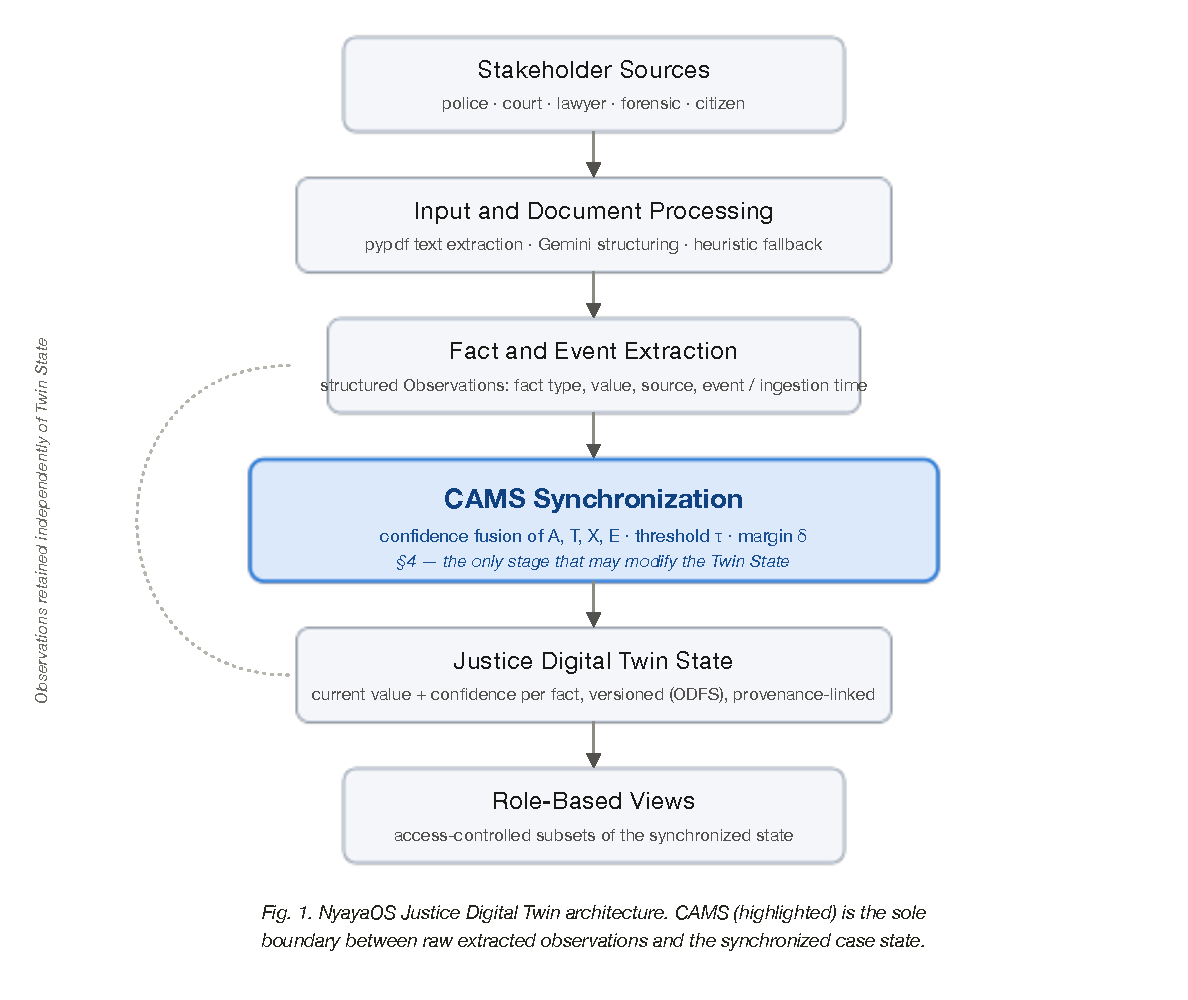
\includegraphics[width=0.85\linewidth]{figures_pdf/fig1_architecture.pdf}
\caption{NyayaOS Justice Digital Twin architecture. CAMS is the sole
boundary between raw extracted observations and the synchronized case
state.}
\label{fig:architecture}
\end{figure}

Information originates from Stakeholder Sources --- police, courts,
lawyers, forensic agencies, and, where authorized, citizens --- each of whom
may report on the same case independently and at different times. Input and
Document Processing turns whatever a source submits (currently,
text-bearing PDF documents) into extracted text, which Fact and Event
Extraction structures into individual Observations: a case identifier, an
entity, a fact type, a candidate value, a source role, an
extraction-reliability estimate, and, where available, the time the
underlying event occurred as distinct from the time the observation was
ingested. Every extracted observation is evaluated by CAMS Synchronization
before it is allowed to change anything else in the system. This is the
only architectural boundary at which the case's synchronized state can be
modified, and Section~\ref{sec:cams} is devoted entirely to what happens
inside it. Whatever CAMS decides, the result is reflected in the Justice
Digital Twin State --- the current, versioned value of each tracked case
fact, together with its confidence and a pointer back to the observation
and decision that produced it --- and consumers see that state only through
Role-Based Views, which restrict which facts a given stakeholder role may
read without altering the underlying synchronized representation.

Two design decisions in this architecture are load-bearing enough to
justify explicitly. First, observations are kept separate from, and are
never deleted or overwritten by, the synchronized Twin State. An incoming
report that conflicts with the current state, or that CAMS judges too weak
to act on, is still stored; it simply does not (yet) change what the Twin
State reports as current. This means the historical record of everything
ever reported about a case survives independently of whatever the system
currently believes, which matters both for auditability and for the
possibility that a later observation resolves an earlier conflict. Second,
an observation's event time --- when the underlying real-world event
occurred --- is recorded separately from its ingestion time --- when the
system received it. Without this separation, a record that happens to
arrive late is indistinguishable from one that describes a late-occurring
event, and a synchronization mechanism has no way to avoid treating "most
recently received" as a proxy for "most currently true." Keeping the two
timestamps distinct is what allows CAMS's temporal-consistency factor
(Section~\ref{sec:cams}) to penalize an observation for describing an event
out of chronological order without penalizing it merely for having arrived
after other records.

Every synchronization decision CAMS makes --- which candidates were
considered, what each factor evaluated to, what the resulting confidence
and margin were, and what was decided --- is stored alongside the
observations it was computed from. This provenance record is what makes a
synchronized fact in the Twin State traceable back to specific evidence
rather than being an opaque current value, and it is what
Section~\ref{sec:method}'s evaluation methodology and
Section~\ref{sec:results}'s results are ultimately built from: nothing
reported in this paper's evaluation is a number computed outside the system
and pasted in --- it is read directly out of this provenance trail.

\section{Confidence-Aware Multi-Source Synchronization}
\label{sec:cams}

CAMS is the mechanism that decides, for each incoming observation, whether
the Justice Digital Twin's synchronized state should change. It is
deliberately narrow in what it decides: CAMS produces a confidence score
used to compare competing \emph{observations of the same fact}, not an
assessment of legal truth, evidentiary admissibility, judicial certainty,
or the correctness of a legal outcome. A high CAMS confidence means an
observation is well-supported enough, relative to its competitors, to be
reflected in the digital representation of the case; it does not mean the
underlying claim is legally established, and NyayaOS does not use it to
make or recommend a judicial decision.

Fig.~\ref{fig:workflow} shows the full decision pipeline. When an
observation is ingested, CAMS first identifies the case, entity, and fact
type it concerns and retrieves every other observation already on record
for that exact combination --- these form the candidate set for
comparison. If this is the first observation ever received for that fact,
there is nothing to compare it against beyond the threshold itself.
Otherwise, every candidate in the set --- the new observation and whichever
prior observations still compete with it --- is scored on four factors and
ranked, and the top two scores determine the outcome.

\begin{figure}[t]
\centering
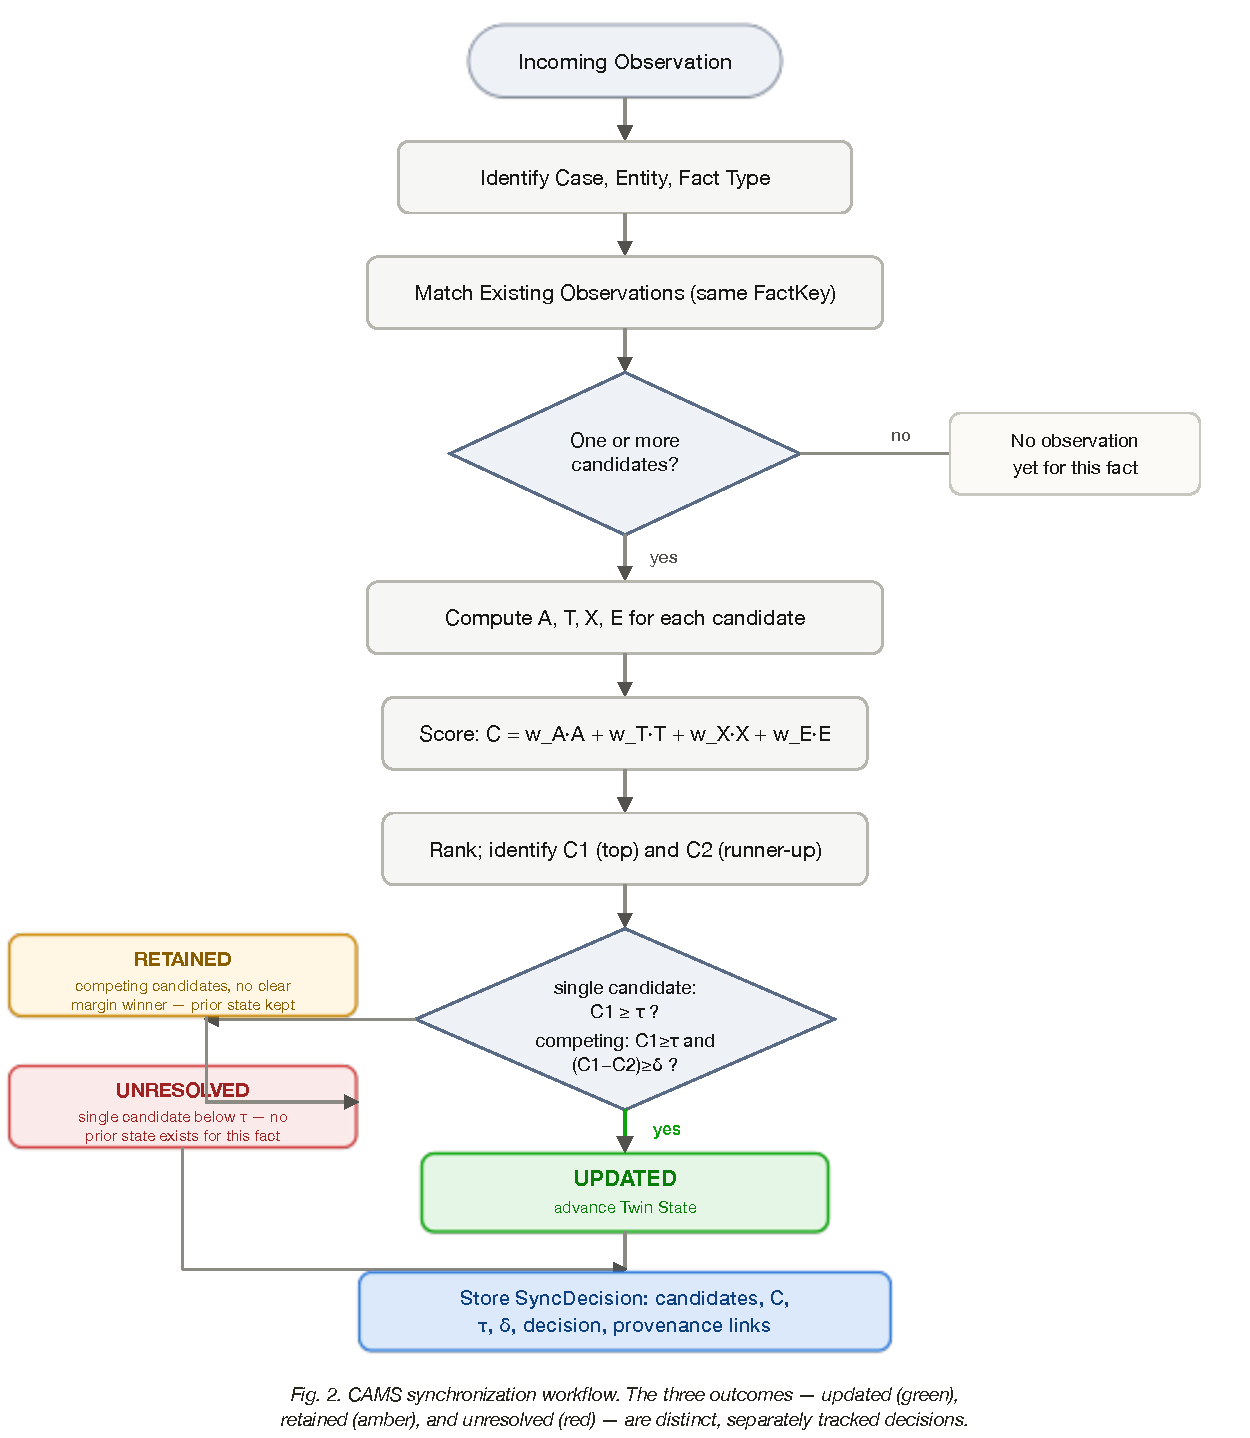
\includegraphics[width=0.95\linewidth]{figures_pdf/fig2_cams_workflow.pdf}
\caption{CAMS synchronization workflow, showing the three possible outcomes
--- updated, retained, and unresolved --- as distinct decisions.}
\label{fig:workflow}
\end{figure}

The four factors are, conceptually, answers to four separate questions
about a candidate observation, computed independently before they are
combined into one number:

\begin{itemize}
\item \textbf{Source authority ($A$)} asks how much weight this \emph{kind}
of source deserves for this \emph{kind} of fact. CAMS does not assume any
single source is authoritative for everything; authority is configured per
(fact type, source role) pair. In the implemented system, a court order
carries higher authority than a police report for bail status (0.95 vs.
0.55), while a forensic laboratory carries the highest authority for a
forensic finding (0.95) and a police report for the same fact type is
weighted much lower (0.45); an unconfigured (fact type, role) pair defaults
to a neutral 0.5. This lets the same source role be treated differently
depending on what it is reporting, rather than imposing one global source
hierarchy.
\item \textbf{Temporal consistency ($T$)} asks whether the event the
observation describes is compatible with what the case's chronology already
establishes, using the event time recorded on the observation rather than
when it happened to arrive. An observation whose event time is at or after
the case's current chronology anchor is fully consistent; one that
describes an event further in the past than that anchor is penalized in
proportion to how far out of order it is, so that a record which simply
arrived late is not automatically treated as describing something that
happened later. When an event time is unavailable for either the candidate
or the anchor, $T$ takes a neutral value rather than being treated as
either consistent or contradictory.
\item \textbf{Cross-source corroboration ($X$)} asks whether a candidate
value is supported by more than one independent source. Multiple
observations from the same source group do not increase $X$ --- the
mechanism specifically counts \emph{distinct} agreeing source groups, so
that one institution repeating itself is not mistaken for independent
confirmation, while genuinely independent agreement (for example, a court,
a police report, and a lawyer's filing all reporting the same status)
increases confidence in proportion to how many distinct groups agree.
\item \textbf{Extraction reliability ($E$)} asks how much to trust the
process that turned a source document into this structured observation,
independently of how authoritative the source itself is. A value typed
directly into a structured field carries full reliability; a value
extracted from a document by an automated pipeline carries whatever
reliability that pipeline reports, keeping "was this correctly read off the
page" separate from "is this source trustworthy."
\end{itemize}

Formally, let $F = \{f_1, \dots, f_n\}$ be the set of candidate
observations competing for the same case fact. For each candidate $f_i$,
CAMS computes four normalized factors $A_i, T_i, X_i, E_i \in [0,1]$ and
combines them as
\begin{equation}
C(f_i) = w_A A_i + w_T T_i + w_X X_i + w_E E_i
\label{eq:score}
\end{equation}
where the weights are non-negative and configured to sum to one,
\begin{equation}
w_A + w_T + w_X + w_E = 1.
\label{eq:weights}
\end{equation}

The implemented system's four factors are computed as follows. Source
authority is a direct table lookup,
\begin{equation}
A_i = A(\text{fact\_type}, \text{source\_role}),
\label{eq:authority}
\end{equation}
defaulting to 0.5 when the pair is not explicitly configured. Temporal
consistency compares the observation's event time $e_i$ against the case's
current chronology anchor $a$ (the event time of the fact's last
synchronized value, when one exists):
\begin{equation}
T_i =
\begin{cases}
1.0, & e_i \ge a \\[2pt]
\max\!\left(0,\; 1 - \dfrac{a - e_i}{30\text{ days}}\right), & e_i < a \\[6pt]
0.5, & e_i \text{ or } a \text{ unavailable}
\end{cases}
\label{eq:temporal}
\end{equation}
so that lateness is penalized continuously rather than as a single binary
contradiction, with the penalty reaching zero once an observation is
roughly a month out of chronological order. Cross-source corroboration
counts $s_i$, the number of distinct source groups whose observations
agree with candidate $f_i$'s value, and saturates at a configured cap
$S_{\max}$ (three in the current configuration):
\begin{equation}
X_i = \min\!\left(1,\; \frac{s_i}{S_{\max}}\right).
\label{eq:corroboration}
\end{equation}
Extraction reliability is a direct pass-through of the reliability value
attached to the observation, clamped to $[0,1]$ and defaulting to 1.0 for
manually entered or already-structured input:
\begin{equation}
E_i \in [0,1].
\label{eq:extraction}
\end{equation}

Given these scores, the candidate with the highest confidence is the
provisional winner,
\begin{equation}
f^{*} = \arg\max_{f_i \in F} C(f_i),
\label{eq:argmax}
\end{equation}
but whether that candidate is actually allowed to update the Twin State
depends on a threshold $\tau$ and, when more than one candidate exists, a
margin $\delta$ as well. Writing $C_1$ for the highest confidence and $C_2$
for the second-highest among competing candidates, the update condition is
\begin{equation}
\text{UPDATE} \iff C_1 \ge \tau \;\wedge\; (C_1 - C_2) \ge \delta
\label{eq:decision}
\end{equation}
when two or more candidates compete, and simply $C_1 \ge \tau$ when only
one candidate exists (there is no runner-up to require a margin against).
The implemented system's default configuration uses $w_A = 0.3$, $w_T =
0.3$, $w_X = 0.2$, $w_E = 0.2$, $\tau = 0.6$, and $\delta = 0.1$.

When the update condition holds, the winning candidate's value becomes the
Twin State's new current value for that fact, its confidence is recorded,
and a new append-only version is written to the fact's version history.
When it does not, the implementation distinguishes two outcomes that the
original design description collapsed into one: if the fact already had a
synchronized value, that value is \textbf{retained} and the competing
candidates are left on record as unresolved competitors; if the fact has
never been synchronized before --- a single candidate that simply failed to
clear $\tau$ --- there is no prior value to fall back on, and the fact is
marked \textbf{unresolved}. Both cases leave every observation intact and
store a full decision record; the difference between them is only whether a
previously synchronized value exists to be preserved.
Fig.~\ref{fig:workflow} shows this branch explicitly, and
Section~\ref{sec:results} reports concrete instances of both.

Ablating a single factor --- used in this paper's
Section~\ref{sec:results} evaluation to test whether each factor actually
matters --- is implemented by fixing that factor's weight to zero and
renormalizing the remaining three so they still sum to one,
\begin{equation}
w_j = 0, \qquad \sum_{k \ne j} w_k = 1,
\label{eq:ablation}
\end{equation}
which changes only how much each remaining factor influences $C$, not the
factors' definitions themselves. Because the candidate set for a given fact
is typically small (bounded by the number of stakeholders who have reported
on it, not by the size of the case as a whole), computing all four factors
and ranking $n$ candidates is linear in $n$, or $O(n \log n)$ if the
implementation additionally sorts the full ranking rather than just
extracting the top two; this is a straightforward property of the
scoring-and-ranking procedure and was not separately benchmarked in this
work.

Fig.~\ref{fig:confidence} illustrates this scoring stage on its own: the
four factors feed the weighted sum of Eq.~(\ref{eq:score}), candidates are
ranked, and the threshold/margin test of Eq.~(\ref{eq:decision}) determines
whether the Twin State is updated or the prior state is retained/marked
unresolved. Where Fig.~\ref{fig:workflow} shows the full decision workflow
including candidate matching and provenance storage, Fig.~\ref{fig:confidence}
is a zoomed-in view of the arithmetic performed inside a single box of that
workflow.

\begin{figure}[t]
\centering
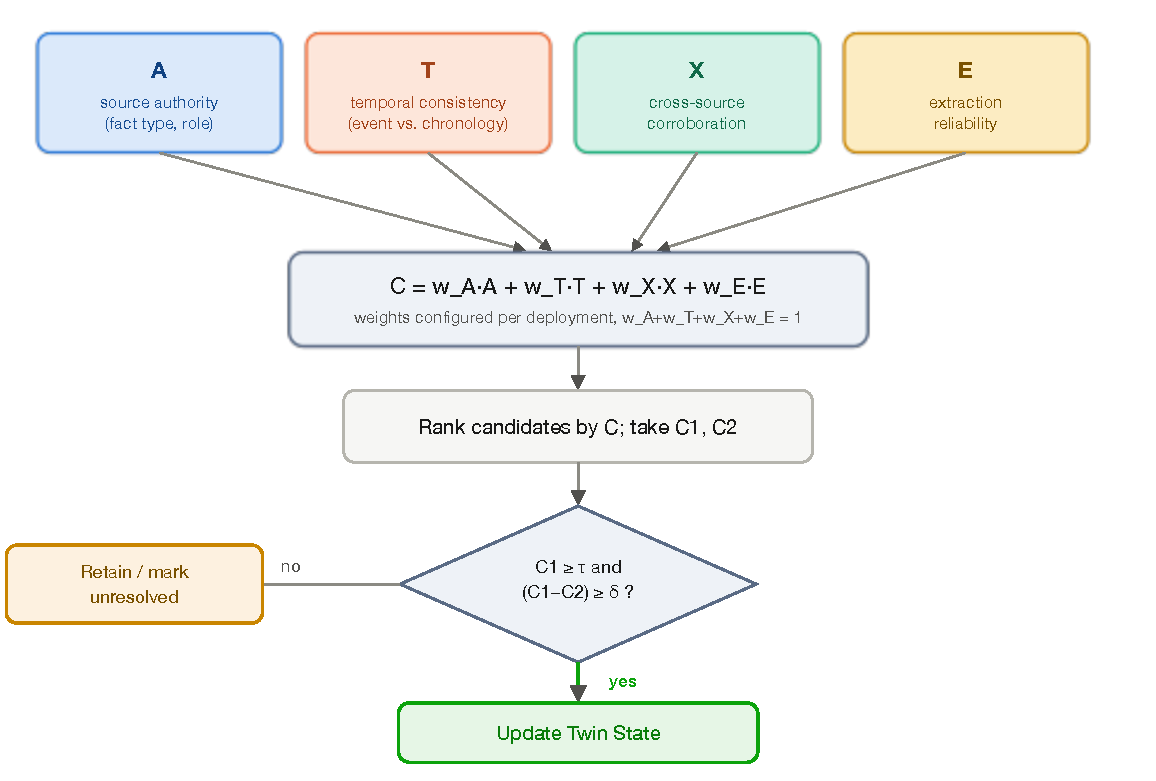
\includegraphics[width=0.95\linewidth]{figures_pdf/fig3_confidence_computation.pdf}
\caption{Confidence computation: the four factors flow into the weighted
sum, and the resulting ranked confidences feed the threshold/margin
synchronization decision.}
\label{fig:confidence}
\end{figure}

A tie between the top two candidates ($C_1 = C_2$) fails the margin
condition in Eq.~(\ref{eq:decision}) whenever $\delta > 0$, so CAMS does
not arbitrarily break ties between equally-supported competing values ---
this is exactly the behavior Section~\ref{sec:results} demonstrates on a
duplicate-observation scenario. We note for precision that this only holds
when $\delta$ is strictly positive; at $\delta = 0$ exactly, a tie
technically satisfies $(C_1 - C_2) \ge \delta$ and would be resolved in
favor of whichever candidate the implementation ranks first. The system's
actual default, $\delta = 0.1$, is comfortably clear of this edge case, but
it is a precise boundary condition rather than an incidental implementation
detail, and Section~\ref{sec:results}.D reports where it was found.

\section{Implementation}

NyayaOS is implemented as a modular Python backend built on FastAPI, with
SQLAlchemy's asynchronous ORM for persistence (PostgreSQL in the intended
deployment; SQLite in the test suite and the demonstration script used for
this paper's evaluation) and Pydantic for request/response validation. The
implementation is organized around the architectural separation described
in Section~\ref{sec:cams}: case and entity records, append-only
observations, the synchronized Twin State and its version history, and CAMS
synchronization decisions are distinct persistence layers, connected by
foreign keys rather than collapsed into a single mutable table.

Document handling extracts text from PDF documents using \texttt{pypdf},
then passes the extracted text to a structuring step that produces the
fact-name, candidate-value, and extraction-reliability fields an
observation needs. This step calls Google's Gemini model through the
\texttt{google-genai} SDK when an API key is configured, and falls back to
a deterministic keyword-matching heuristic when it is not --- a fallback
that is scientifically relevant, since it determines the
extraction-reliability value ($E$) attached to the resulting observation,
and is therefore reported here rather than left implicit. Scanned or
image-only documents are not currently supported: the text-extraction step
raises an explicit error for a PDF with no extractable text layer, since no
OCR component is implemented. This is stated plainly as a current
limitation of the document-processing stage, not implied to be handled.

The CAMS engine itself (factor computation, confidence fusion, and the
threshold/margin decision rule of Section~\ref{sec:cams}) is implemented as
a small, dependency-free module that takes plain data structures in and
returns a decision object out, independent of the database and web layers;
this is what allows it to be exercised directly by unit tests and by the
evaluation harness in Section~\ref{sec:method} without standing up a
database or an HTTP server. The observation service that sits above it is
the integration point that resolves a fact's existing candidates from
storage, invokes the CAMS engine, and --- only when the engine's decision
is \texttt{updated} --- advances the Twin State and appends a new version to
that fact's history; every invocation, regardless of outcome, writes a
synchronization-decision record carrying the candidates considered, their
computed factors and confidence, the threshold and margin used, and the
decision reached. FastAPI routes expose case and entity management,
observation ingestion, and Twin State retrieval, documented through the
framework's built-in OpenAPI interface; the corresponding evaluation
endpoint intended to trigger the harness of Section~\ref{sec:method} over
the API was not implemented at the time of this audit and is not relied on
here --- this paper's evaluation was run directly against the underlying
modules instead, as described in Section~\ref{sec:method}.

\section{Experimental Methodology}
\label{sec:method}

This paper's evaluation is built entirely from executions of the
implemented system, verified against its source code rather than assumed
from its description. Three pieces of evidence are used, each addressing a
different question, and none of them supports claims beyond what it
actually measures.

The first is the existing automated test suite: 14 unit tests exercising
the CAMS engine and factor calculator in isolation, and 9 integration tests
exercising observation ingestion, synchronization, and Twin
State/version-history behavior through the actual API and database layer,
covering conflicting, delayed, duplicate, corroborated, noisy, and
low-confidence observations. These establish that the implementation
behaves as Section~\ref{sec:cams} describes it, under the specific
conditions each test constructs; they are a correctness check on the
mechanism, not an evaluation of its behavior on realistic case data.

The second is an end-to-end pipeline execution: a demonstration script,
already present in the repository and not written for this paper, that
creates one case and one entity, and ingests a sequence of nine
observations from four stakeholder roles (court, police, lawyer, forensic)
covering three fact types (\texttt{bail\_status}, \texttt{forensic\_result},
\texttt{identity}), each ingestion invoking the same observation service
and CAMS engine a real API call would use. This exercises the full
pipeline --- ingestion, factor computation, synchronization decision, Twin
State update or retention, and version history --- on one continuous case
narrative, and is the source of Section~\ref{sec:results}.A's pipeline-level
numbers and Section~\ref{sec:results}.B's worked examples.

The third is a controlled comparative evaluation, built by completing an
evaluation harness that existed in the repository only as scaffolding (four
of five scenario generators, and the harness's baseline/ablation loop, were
unimplemented placeholders at the time of this audit; see the accompanying
audit document for exactly what was already present versus completed for
this paper). Five scenario types were defined --- conflicting, delayed,
noisy, corroborating, and duplicate observations --- each as a small,
hand-constructed set of candidate observations with a pre-specified
reference value representing the outcome the mechanism is intended to
reach. Eight synchronization methods were then run against every scenario:
CAMS with its full default configuration; four ablations of CAMS, each with
exactly one factor's weight zeroed and the remaining three renormalized per
Eq.~(\ref{eq:ablation}); and three simpler baseline rules already present in
the repository as separate modules --- a fixed global source-authority
hierarchy, a rule that always prefers the most recently ingested
observation regardless of confidence, and a simple majority vote over
candidate values. For each (scenario, method) pair we recorded the
predicted value, the resulting decision, and whether the predicted value
matched the scenario's reference value. We report this match rate as a
\textbf{value-match rate}, not as accuracy in a classification-benchmark
sense: the scenarios are small, hand-authored, and designed to isolate one
mechanism at a time, not sampled from or representative of real case data,
and a value-match rate computed over five scenarios is a diagnostic of
mechanism behavior, not a statistically powered accuracy estimate.

Finally, a threshold/margin sensitivity sweep was run directly against the
CAMS engine, varying $\tau$ over $[0.30, 0.90]$ with $\delta$ fixed at its
default of $0.1$, and varying $\delta$ over $[0.00, 0.30]$ with $\tau$
fixed at its default of $0.6$, recording the decision boundary --- the
parameter value at which the outcome for a given scenario flips from
\texttt{updated} to \texttt{retained} --- for each of the five scenarios
above.

All three pieces of evidence were executed with \texttt{DATABASE\_URL}
pointed at an in-memory SQLite database (avoiding any dependency on a
running PostgreSQL instance) against the repository's \texttt{main} branch,
and their raw console output was saved verbatim as
\texttt{paper/evidence/demo\_person\_c\_output.txt},
\texttt{paper/evidence/eval\_comparison\_report.txt}, and
\texttt{paper/evidence/sensitivity\_sweep\_report.txt} respectively. Every
number in Section~\ref{sec:results} is read directly from one of these
three files.

\section{Results and Analysis}
\label{sec:results}

\subsection{End-to-end pipeline execution}

Table~\ref{tab:pipeline} summarizes the demonstration run described in
Section~\ref{sec:method}. Nine observations were ingested across three
fact types; each ingestion triggered one CAMS synchronization decision, so
nine decisions were made in total. Seven resulted in the Twin State being
updated, one in the prior state being retained, and one in the fact being
left unresolved because no prior state existed for it to fall back on. Two
Digital Twin facts were maintained by the end of the run
(\texttt{bail\_status} and \texttt{forensic\_result}); the third fact type
touched (\texttt{identity}) never reached a synchronized value, because its
only observation did not clear the confidence threshold. The
\texttt{bail\_status} fact accumulated five append-only version-history
entries and \texttt{forensic\_result} two, reflecting every time a
competing or corroborating observation caused CAMS to recompute and
re-affirm (or change) the synchronized value.

\begin{table}[t]
\centering
\caption{End-to-end pipeline execution (single demonstration run)}
\label{tab:pipeline}
\rowcolors{2}{rowstripe}{white}
\begin{tabular}{L{5.2cm}C{2cm}}
\toprule
\rowcolor{headerfill}
\textcolor{headertext}{\textbf{Metric}} & \textcolor{headertext}{\textbf{Result}} \\
\midrule
Case documents / scenario & 1 case, 4 roles \\
Observations ingested & 9 \\
Fact types touched & 3 \\
CAMS synchronization decisions & 9 \\
\quad--- updated & 7 \\
\quad--- retained & 1 \\
\quad--- unresolved & 1 \\
Twin facts synchronized by end of run & 2 of 3 \\
\texttt{bail\_status} version history length & 5 \\
\texttt{forensic\_result} version history length & 2 \\
\bottomrule
\end{tabular}
\end{table}

This is not the scale of a production system, and it is not presented as
one; it is a verification that the full pipeline --- from ingestion through
synchronization to versioned, provenance-linked state --- executes as
Section~\ref{sec:architecture} and Section~\ref{sec:cams} describe, on real
(if small) input.

\subsection{Representative synchronization decisions}

Six decisions from the same run illustrate how the mechanism behaves,
using its actual computed values rather than illustrative numbers.

The first observation of the run --- a court filing of
\texttt{bail\_status = granted} --- has no prior competitor. With no
established chronology yet, its temporal factor takes the neutral value
$T=0.5$; its authority is $A=0.95$ (court is the highest-authority source
for bail status in the configured table), corroboration is $X=0.0$ (a
single observation cannot corroborate itself), and extraction reliability
is $E=1.0$ (structured input). This gives $C = 0.3(0.95) + 0.3(0.5) +
0.2(0.0) + 0.2(1.0) = 0.635$, which clears $\tau = 0.6$, so the fact is
synchronized with confidence 0.635 and no runner-up.

When police and then a lawyer independently file the same value
(\texttt{granted}), corroboration rises as each additional independent
source group agrees --- $X$ moves from 0.0 to 0.333 (one corroborating
group) to 0.667 (two) --- and the court observation's confidence rises
correspondingly to 0.852 and then 0.918, while the newer, lower-authority
observations remain ranked below it. Because the top candidate's margin
over the runner-up stays above $\delta=0.1$ throughout, each of these
observations still results in \texttt{updated}, appending a new,
higher-confidence version to the fact's history even though the
synchronized \emph{value} does not change --- a version records a
reaffirmation of the existing value, not only a change of value.

When police subsequently reports a conflicting value (\texttt{denied}),
that observation scores $C=0.665$ --- still below the court-corroborated
candidate's 0.918 by a margin of 0.253 --- so the synchronized value
remains \texttt{granted}; the conflicting observation is preserved as a
competing, unresolved candidate rather than discarded. A later police
observation reporting \texttt{in\_custody}, whose event time is 25 days
before the case's chronology anchor, scores even lower ($T=0.167$ under the
temporal-decay rule of Eq.~(\ref{eq:temporal}), giving $C=0.415$) and loses
for the same structural reason: being ingested later does not make an
out-of-order event time consistent.

A duplicate filing of the original court observation --- same source, same
value --- ties the existing top candidate exactly ($C_1 = C_2 = 0.918$).
Because the margin condition requires $C_1 - C_2 \ge \delta = 0.1$ and the
margin here is zero, CAMS does not select either candidate; the decision is
\texttt{retained}, the Twin State is untouched, and the duplicate is stored
only for audit. This is the duplicate-tie behavior Section~\ref{sec:cams}
describes formally.

Finally, a single low-reliability observation reporting a possible
identity (\texttt{extraction\_reliability = 0.15}) scores $C = 0.33$, well
below $\tau = 0.6$. Because no \texttt{identity} fact had ever been
synchronized before, there is no prior value to retain --- the decision is
\texttt{unresolved}, and no Digital Twin fact for \texttt{identity} is
created. This is the case this paper uses to illustrate abstention: CAMS
explicitly withholds a synchronized value rather than accepting a weakly
supported one, and the underlying observation remains on record for a
future, better-supported observation to resolve.

Fig.~\ref{fig:trajectory} plots this entire sequence as one continuous
trace of the \texttt{bail\_status} fact's synchronized confidence, alongside
every competing observation that was evaluated and lost. The solid line
tracks the Twin State's confidence after each of the five observations that
resulted in \texttt{updated}; the hollow diamond at step 6 marks the
duplicate observation, whose tied score left the Twin State unchanged
(\texttt{retained}) rather than advancing it to a sixth version. The two
crosses below the $\tau=0.6$ line are the conflicting and delayed
observations from steps 4 and 5: both were evaluated, both lost, and
neither was discarded --- they remain visible in this figure precisely
because they were preserved as competing candidates rather than deleted.
Reading the figure left to right makes the shape of Section~\ref{sec:cams}'s
mechanism concrete: confidence climbs as independent corroboration
accumulates (steps 1--3), plateaus once no further corroboration is offered
(step 4), and a weak or out-of-order competitor never comes close to
disturbing it (steps 4--5) until an exact tie is reached, at which point the
mechanism deliberately stops rather than picking a winner (step 6).

\begin{figure}[t]
\centering
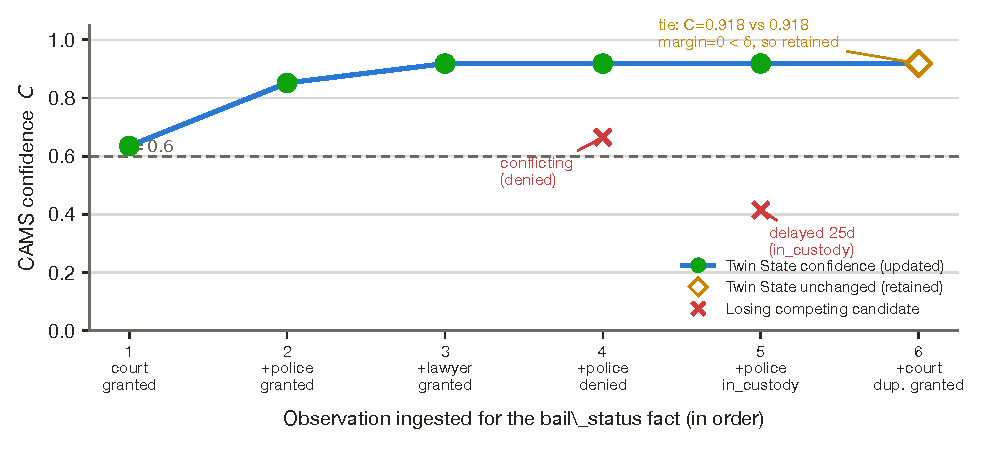
\includegraphics[width=\linewidth]{figures_pdf/fig4_confidence_trajectory.pdf}
\caption{Confidence trajectory across the six observations ingested for one
\texttt{bail\_status} fact in the end-to-end demonstration run. Green
circles are accepted updates; the amber diamond is a retained tie; red
crosses are losing competing candidates preserved as unresolved history.}
\label{fig:trajectory}
\end{figure}

\subsection{Comparative evaluation: CAMS, ablations, and baselines}

Table~\ref{tab:comparison} reports the value-match rate
(Section~\ref{sec:method}) for CAMS and seven comparison methods across the
five controlled scenarios. CAMS's full configuration matched the reference
outcome in 4 of 5 scenarios (80\%); the only mismatch is the duplicate
scenario, where CAMS reports no winner by design (Section~\ref{sec:cams})
rather than an incorrect value --- a behavioral difference from the other
four scenarios, not a value error, and discussed further in
Section~\ref{sec:discussion}.

\begin{table*}[t]
\centering
\caption{Value-match rate: CAMS, ablations, and baselines across five scenarios}
\label{tab:comparison}
\rowcolors{2}{rowstripe}{white}
\begin{tabular}{lccccccc}
\toprule
\rowcolor{headerfill}
\textcolor{headertext}{\textbf{Method}} & \textcolor{headertext}{\textbf{Conflicting}} & \textcolor{headertext}{\textbf{Delayed}} & \textcolor{headertext}{\textbf{Noisy}} & \textcolor{headertext}{\textbf{Corroboration}} & \textcolor{headertext}{\textbf{Duplicate}} & \textcolor{headertext}{\textbf{Match rate}} \\
\midrule
CAMS (full) & \okmark & \okmark & \okmark & \okmark & --- (retained) & 4/5 (80\%) \\
CAMS $-$ A (authority ablated) & \okmark & \okmark & \okmark & \okmark & --- (retained) & 4/5 (80\%) \\
CAMS $-$ T (temporal ablated) & \okmark & \badmark & \okmark & \okmark & --- (retained) & 3/5 (60\%) \\
CAMS $-$ X (corroboration ablated) & \okmark & \okmark & \okmark & \badmark & --- (retained) & 3/5 (60\%) \\
CAMS $-$ E (extraction ablated) & \okmark & \okmark & \badmark & \okmark & --- (retained) & 3/5 (60\%) \\
Fixed source-authority hierarchy & \okmark & \okmark & \okmark & \okmark & \okmark & 5/5 (100\%)$^{*}$ \\
Latest-ingestion-wins & \badmark & \badmark & \badmark & \okmark & \okmark & 2/5 (40\%) \\
Majority voting & \okmark & \okmark & \okmark & \badmark & \okmark & 4/5 (80\%) \\
\bottomrule
\end{tabular}

\vspace{2pt}
\footnotesize $^{*}$See Section~\ref{sec:discussion}: this scenario set was not designed to be adversarial to a fixed hierarchy, and this result should not be read as general evidence that a fixed hierarchy is sufficient.
\end{table*}

Each single-factor ablation failed precisely the scenario constructed to
exercise that factor: removing temporal consistency ($w_T=0$) caused CAMS
to fail the delayed-observation scenario (it retains rather than correctly
preferring the temporally-consistent candidate); removing corroboration
($w_X=0$) caused it to fail the corroboration scenario; removing extraction
reliability ($w_E=0$) caused it to fail the noisy-observation scenario.
Removing authority ($w_A=0$) did not introduce a new failure in this
scenario set --- the conflicting scenario's winning candidate happened to
be favored by its other three factors as well, so this result should be
read as "authority was not the deciding factor in these particular
scenarios," not as evidence that authority is dispensable in general. The
naive latest-ingestion-wins baseline performed worst overall (2/5), failing
every scenario in which the temporally, evidentially, or reliability-wise
weaker observation happened to be ingested last --- exactly the failure
mode Section~\ref{sec:introduction} motivates CAMS against.

Fig.~\ref{fig:matchrate} presents the same eight match rates from
Table~\ref{tab:comparison} as a single ranked comparison, which is easier to
scan for the overall pattern than the per-scenario grid: the four ablations
cluster visibly below the full CAMS configuration, confirming that removing
any one of the three factors that matter in this scenario set costs a full
scenario's worth of accuracy, while the three baselines spread across the
full range from worst (latest-ingestion-wins) to nominally best
(fixed-authority) performer overall. The asterisk on the fixed-authority bar
is deliberate and carries into the figure the same caveat given for
Table~\ref{tab:comparison} and expanded in Section~\ref{sec:discussion}: that
result reflects this scenario set's design, not a general finding that a
static hierarchy is adequate.

\begin{figure}[t]
\centering
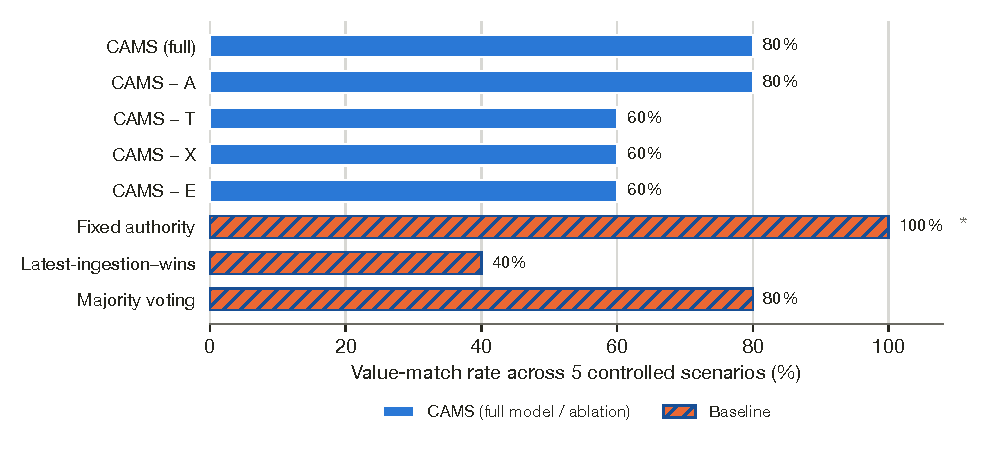
\includegraphics[width=\linewidth]{figures_pdf/fig5_match_rate.pdf}
\caption{Value-match rate by method, aggregated from Table~\ref{tab:comparison}.
CAMS and its ablations (blue) cluster together; the three baselines (orange,
hatched) span the full range from worst to nominally best on this scenario set.}
\label{fig:matchrate}
\end{figure}

\subsection{Threshold and margin sensitivity}

Table~\ref{tab:sensitivity} reports, for each scenario, the highest value
of $\tau$ (with $\delta=0.1$ fixed) and the highest value of $\delta$ (with
$\tau=0.6$ fixed) at which the scenario still resolves to \texttt{updated},
together with the margin $C_1-C_2$ each scenario actually produces at the
default configuration.

\begin{table}[t]
\centering
\caption{Decision-boundary sensitivity (sweep over $\tau \in [0.30,0.90]$, $\delta \in [0.00,0.30]$)}
\label{tab:sensitivity}
\rowcolors{2}{rowstripe}{white}
\begin{tabular}{L{2.1cm}C{1.5cm}C{1.5cm}C{1.4cm}}
\toprule
\rowcolor{headerfill}
\textcolor{headertext}{\textbf{Scenario}} & \textcolor{headertext}{\textbf{Updated while $\tau \le$}} & \textcolor{headertext}{\textbf{Updated while $\delta \le$}} & \textcolor{headertext}{\textbf{Margin at default}} \\
\midrule
Conflicting & 0.85 & $\ge$0.30 & 0.48 \\
Delayed & 0.80 & 0.24 & 0.24 \\
Noisy & 0.70 & 0.14 & 0.16 \\
Corroboration & 0.75 & 0.18 & 0.20 \\
Duplicate & never$^{\dagger}$ & 0.00 only & 0.00 \\
\bottomrule
\end{tabular}

\vspace{2pt}
\footnotesize $^{\dagger}$Margin is 0 for this scenario, so no $\tau$ in the swept range produces \texttt{updated} once $\delta > 0$.
\end{table}

The scenarios are not equally robust to the choice of parameters: the
conflicting and delayed scenarios tolerate a wide range of $\tau$ and
$\delta$ before their outcome would flip, while the noisy and corroboration
scenarios are comparatively closer to their decision boundary at the
system's default configuration ($\tau=0.6,\delta=0.1$), margins of 0.16 and
0.20 respectively against a required $\delta=0.1$. The duplicate scenario
never resolves to \texttt{updated} anywhere in the swept range once
$\delta>0$, confirming the tie behavior described formally in
Section~\ref{sec:cams}; the one exception, at exactly $\delta=0.00$, is the
boundary condition noted there --- a tie is only ever resolved when the
margin requirement is disabled entirely, which is not the system's
configured default.

Fig.~\ref{fig:sensitivity} shows the $\tau$ half of Table~\ref{tab:sensitivity}
as a range per scenario, which makes the unevenness in robustness easier to
see at a glance than the table's raw numbers: each bar spans from the
sweep's lower bound to the exact $\tau$ at which that scenario's outcome
flips from \texttt{updated} to \texttt{retained}, and the dashed vertical
line marks the system's configured default, $\tau=0.6$. The conflicting
scenario's bar reaches nearly to the top of the swept range, meaning its
outcome is essentially insensitive to reasonable choices of $\tau$; the
noisy and corroboration scenarios' bars end closer to the default line,
meaning a modestly stricter threshold would flip their outcome. The
duplicate scenario has no bar at all --- consistent with
Table~\ref{tab:sensitivity}, its margin is zero regardless of $\tau$, so
$\tau$ alone can never make it resolve to \texttt{updated}.

\begin{figure}[t]
\centering
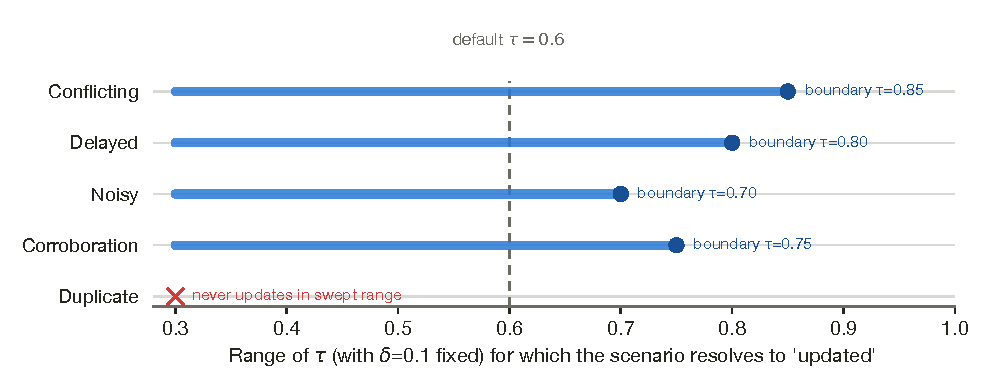
\includegraphics[width=\linewidth]{figures_pdf/fig6_sensitivity_range.pdf}
\caption{Range of $\tau$ (with $\delta=0.1$ fixed) over which each scenario
resolves to \texttt{updated}, from the sweep underlying Table~\ref{tab:sensitivity}.
The dashed line marks the system's configured default, $\tau=0.6$.}
\label{fig:sensitivity}
\end{figure}

\section{Discussion}
\label{sec:discussion}

The evaluation in Section~\ref{sec:results} demonstrates that the
implemented mechanism does what Section~\ref{sec:cams} describes: it
distinguishes observations that should change the synchronized case state
from those that should not, using exactly the four factors it claims to
use, and each factor's removal breaks exactly the case it is meant to
handle. That is a narrower claim than demonstrating that CAMS produces
\emph{correct} case representations in general, and the two should not be
conflated. What the ablation results establish is internal consistency
between the mechanism's design and its implementation, confirmed by
execution rather than by reading the code; they do not establish that the
chosen weights, threshold, or margin are the right ones for any particular
deployment, or that this mechanism would perform comparably on real,
larger, or more adversarial case data.

The comparison against baselines is informative in both directions. CAMS
outperformed a naive latest-ingestion-wins rule by a wide margin (80\% vs.
40\%) on exactly the failure modes --- temporal disorder, noise, weak
corroboration --- that motivate treating confidence as multi-factorial
rather than reducing synchronization to "trust whatever arrived last." It
did not clearly outperform either the fixed-source-authority baseline or
majority voting on this small scenario set, and the fixed-authority
baseline's perfect score deserves a direct caveat rather than a favorable
gloss: the five scenarios were constructed to test CAMS's individual
factors, not to be adversarial to a static authority hierarchy, and in each
of them the reference outcome happened to coincide with what a fixed
court-over-police-over-lawyer ranking would also produce. This is a
property of the evaluation's scenario design, not evidence that a fixed
hierarchy is sufficient in general; a case where the authoritative source
for a fact type is \emph{not} the source a fixed global hierarchy would
rank highest --- exactly the situation CAMS's fact-dependent authority
table (Section~\ref{sec:cams}) is designed to handle, and a fixed hierarchy
structurally cannot --- was not included in this scenario set and would be
a natural next test.

Abstention, illustrated in Section~\ref{sec:results}.B by the
low-confidence identity observation, is a deliberate design choice worth
interpreting explicitly: withholding a synchronized value is treated as an
acceptable and even preferred outcome when the available evidence does not
clear the confidence threshold, rather than the mechanism being forced to
commit to a best-guess value. This only has value because of the
architecture's second commitment, from Section~\ref{sec:architecture} ---
that unresolved or rejected observations are never discarded, only left
unsynchronized --- so an abstention is not a loss of information, only a
deferral, and a stronger future observation can still resolve it. This is
also why the duplicate scenario's "failure" in Table~\ref{tab:comparison}
should be read alongside its description in Section~\ref{sec:results}.A
rather than at face value: CAMS reports no value there because it
correctly recognizes no genuine competing value exists, not because it
failed to recover an available answer.

CAMS's confidence fusion is a weighted linear combination of four
heuristically defined factors, and this simplicity is intentional but
should not be overstated: it is easy to compute, easy to explain, and ---
as the ablation results show --- each term's contribution can be isolated
and tested, but it is not a learned or empirically calibrated model, and
nothing in this paper's evaluation validates the specific weights, the
specific authority values, or the specific 30-day temporal-decay window
against real-world outcomes. The mechanism can fail in ways this evaluation
was not designed to surface: an authority table that is wrong or stale for
a given deployment, a corroboration cap that saturates too early or too
late for how many independent source groups a real case actually has, or a
temporal-decay window mismatched to how quickly a particular kind of case
fact actually changes, would all degrade CAMS's decisions without
necessarily being visible in a scenario set constructed, as this one was,
around the mechanism's intended behavior rather than around its plausible
failure modes.

\section{Limitations and Future Work}

This work's evidentiary base is small and self-constructed by design, and
every limitation below follows from that. The end-to-end execution covers a
single hand-built case with nine observations; the comparative evaluation
covers five scenarios with two candidate observations each. Neither is a
real or independently annotated legal dataset, and no statistical claim ---
a confidence interval, a significance test, an estimate of variance across
cases --- is possible or attempted at this scale. The reference values used
in the comparative evaluation were authored alongside the scenarios that
generate them, in the same way the repository's own unit tests already
construct expected outcomes; they demonstrate that the mechanism reaches
its intended outcome on cases designed to test it, not that its outcomes
would match independent legal or factual judgment on real cases.

The source-authority table and the extraction-reliability values used
throughout are configured engineering priors, not values calibrated against
real case outcomes or validated by legal domain experts; the temporal-decay
rule (a fixed 30-day linear window) is similarly a deterministic design
choice rather than a learned or empirically justified one. The scenario set
used four source roles (court, police, lawyer, forensic) and did not
exercise the fifth configured role (citizen) or scenarios with more than
two competing source groups; conflict diversity was similarly limited to
single-value disagreements, not, for example, scenarios with three or more
mutually inconsistent values or adversarially constructed source
combinations. The evaluation harness's two remaining metrics --- a
conflict-resolution accuracy measure and a confidence-calibration measure
--- were left unimplemented in this session, consistent with their state in
the repository prior to this audit, and are not used in this paper's
results; they remain a concrete, scoped next step rather than a gap papered
over.

At the implementation level, the document-processing stage does not
currently support scanned or image-only documents --- every observation
used in this paper's evaluation was constructed directly as structured
data, not extracted from a real document image through an OCR pipeline, and
the extraction-quality claims this paper can make are limited accordingly.
Finally, this paper makes no claim about deployment readiness, governance,
or legal-process integration: role-based access exists at the level of
authenticated user roles, but the broader questions of how a Justice
Digital Twin would be governed, audited by non-technical stakeholders, or
integrated into an actual judicial workflow were out of scope for this
evaluation.

The most direct next step is evaluating CAMS against a larger,
independently annotated collection of legal cases spanning multiple genuine
source groups, delayed and duplicate records, and deliberately adversarial
conflicts --- including cases constructed specifically to test whether a
fixed source hierarchy is \emph{insufficient}, addressing the asymmetry
noted in Section~\ref{sec:discussion}. Beyond scale, the confidence factors
themselves are a natural target for empirical calibration --- learning or
validating authority values, corroboration caps, and temporal-decay
parameters against real outcomes rather than fixing them by design --- and
the document-processing stage would need a real OCR path before any claim
about scanned-document robustness could be made. Completing the evaluation
harness's remaining metrics, extending role-based views into a fully
differentiated per-stakeholder interface, and examining what
provenance-based auditability looks like from a non-technical user's
perspective are further concrete extensions of this work.

\section{Conclusion}

This paper addressed the problem of maintaining one continuously updated,
internally consistent representation of a legal case when the information
that feeds it is produced independently by multiple stakeholders, arrives
out of order, repeats itself, and sometimes disagrees with itself. It
proposed CAMS, a confidence-aware synchronization mechanism that scores
competing observations of the same case fact on source authority, temporal
consistency, cross-source corroboration, and extraction reliability, and
uses a threshold-and-margin rule to decide whether the synchronized Justice
Digital Twin state should be updated, retained, or left unresolved, with
every decision and every observation preserved for provenance.

What was actually implemented and verified in this work is a working
backend that carries this mechanism end to end --- from document text
extraction through structured observation, synchronization, and versioned,
provenance-linked case state --- confirmed against its own source code and
test suite rather than taken on the strength of its own description. The
evaluation performed here demonstrated that the mechanism behaves as
designed on a small, controlled set of scenarios: it reached its intended
outcome in the large majority of cases tested, each of its four confidence
factors could be shown, by ablation, to be doing real work, and it
distinguished a genuine deferral (abstention) from a resolvable conflict in
a way that a simpler recency-based baseline could not.

What remains unresolved is everything that follows from the evaluation's
small, hand-constructed scale: whether CAMS's specific parameters
generalize to real case data, whether its advantage over simpler baselines
holds on scenarios not designed around its own factors, and whether its
confidence scores would correspond to anything a legal domain expert would
independently agree with. None of this paper's results should be read as
evidence of legal accuracy, production readiness, or fitness to inform an
actual judicial decision --- CAMS governs a digital representation of a
case, not the case itself. The next research step is a larger,
independently annotated, and deliberately adversarial evaluation capable of
testing where this design's assumptions actually break.

\begin{thebibliography}{00}

\bibitem{bhatt2024} H. Bhatt, R. Bahuguna, S. Swami, R. Singh, A. Gehlot, S.
V. Akram, L. R. Gupta, A. K. Thakur, N. Priyadarshi, and B. Twala,
``Integrating industry 4.0 technologies for the administration of courts
and justice dispensation---a systematic review,'' \emph{Humanities and
Social Sciences Communications}, vol. 11, Art. no. 1076, 2024, doi:
10.1057/s41599-024-03587-0.

\bibitem{han2024} W. Han, J. Shen, Y. Liu, Z. Shi, J. Xu, F. Hu, H. Chen, Y.
Gong, X. Yu, X. Yu, H.-Q. Wang, Z. Liu, Y. Yang, T. Shi, and M. Ge,
``LegalAsst: Human-centered and AI-empowered machine to enhance court
productivity and legal assistance,'' \emph{Information Sciences}, vol.
679, Art. no. 121052, 2024, doi: 10.1016/j.ins.2024.121052.

\bibitem{yue2024} L. Yue, Q. Liu, B. Jin, H. Wu, and Y. An, ``A
circumstance-aware neural framework for explainable legal judgment
prediction,'' \emph{IEEE Transactions on Knowledge and Data Engineering},
vol. 36, no. 11, pp. 5453--5467, 2024, doi: 10.1109/TKDE.2024.3387580.

\bibitem{li2024} X. Li, F. Dunkin, and J. Dezert, ``Multi-source
information fusion: Progress and future,'' \emph{Chinese Journal of
Aeronautics}, vol. 37, no. 7, pp. 24--58, 2024, doi:
10.1016/j.cja.2023.12.009.

\bibitem{jiao2024} L. Jiao, ``Advances in uncertain information fusion,''
\emph{Entropy}, vol. 26, no. 11, Art. no. 945, 2024, doi:
10.3390/e26110945.

\bibitem{castano2024} S. Castano, A. Ferrara, E. Furiosi, S. Montanelli, S.
Picascia, D. Riva, and C. Stefanetti, ``Enforcing legal information
extraction through context-aware techniques: The ASKE approach,''
\emph{Computer Law \& Security Review}, vol. 52, Art. no. 105903, 2024,
doi: 10.1016/j.clsr.2023.105903.

\bibitem{habernal2024} I. Habernal, D. Faber, N. Recchia, S. Bretthauer, I.
Gurevych, I. Spiecker genannt D\"{o}hmann, and C. Burchard, ``Mining legal
arguments in court decisions,'' \emph{Artificial Intelligence and Law},
vol. 32, no. 3, pp. 557--594, 2024, doi: 10.1007/s10506-023-09361-y.

\bibitem{bex2025} F. J. Bex, ``AI, Law and beyond. A transdisciplinary
ecosystem for the future of AI \& Law,'' \emph{Artificial Intelligence and
Law}, vol. 33, pp. 253--270, 2025, doi: 10.1007/s10506-024-09404-y.

\bibitem{papagianneas2023} S. Papagianneas and N. Junius, ``Fairness and
justice through automation in China's smart courts,'' \emph{Computer Law
\& Security Review}, vol. 51, Art. no. 105897, 2023, doi:
10.1016/j.clsr.2023.105897.

\bibitem{pfeiffer2023} J. Pfeiffer, J. Gutschow, C. Haas, F. M\"{o}slein, O.
Maspfuhl, F. Borgers, and S. Alpsancar, ``Algorithmic fairness in AI: An
interdisciplinary view,'' \emph{Business \& Information Systems
Engineering}, vol. 65, no. 2, pp. 209--222, 2023, doi:
10.1007/s12599-\emph{[DOI incomplete in source manuscript --- not
independently verified; see audit note]}.

\end{thebibliography}

\vspace{6pt}
\footnotesize\noindent\emph{Note on references.} This reference list is
carried over from the baseline manuscript unchanged in content. Live
DOI/citation verification could not be completed during preparation of this
manuscript (no network access to a citation database was available); DOI
\cite{pfeiffer2023} is truncated in the original source document itself and
is left unfilled here rather than completed with invented digits. All
entries should be manually verified against the publisher record before
submission.

\end{document}
